\documentclass{article}

\usepackage{helvet} %Set default font
\renewcommand{\familydefault}{\sfdefault}

\usepackage[a4paper, margin=25mm]{geometry} %Setting document size and margin width

\usepackage[utf8]{inputenc}
\usepackage[url=false, doi=false, isbn=false, bibstyle=ieee, citestyle=numeric-comp]{biblatex} %Set bibliography style
\addbibresource{Lit_rev.bib} %Imports .bib file

\usepackage{graphicx} %Required for graphics and figures
\graphicspath{ {./Fig/} }
\usepackage[export]{adjustbox} %Used for adjusting image box
\usepackage{caption} %For caption customizations
\usepackage{subcaption}

\title{\textbf{Literature Review \\and \\Lay Summary}}
\author{Jasper Ng}
\date{May 2025}

\begin{document}

\maketitle

\begin{figure}[h]
    \centering
    \begin{subfigure}[c]{0.45\linewidth}
        \centering
        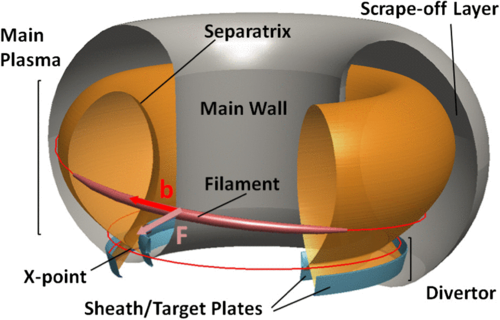
\includegraphics[width=0.9\linewidth]{Fig1_plasma_filament.png}
        \normalsize{\caption{Example of a plasma filament along a magnetic field line in the SOL \cite{carralero_experimental_2015}}}
        \label{fig:fig1}
    \end{subfigure}
    \hspace{0.05\linewidth}
    \begin{subfigure}[c]{0.45\linewidth}
        \centering
        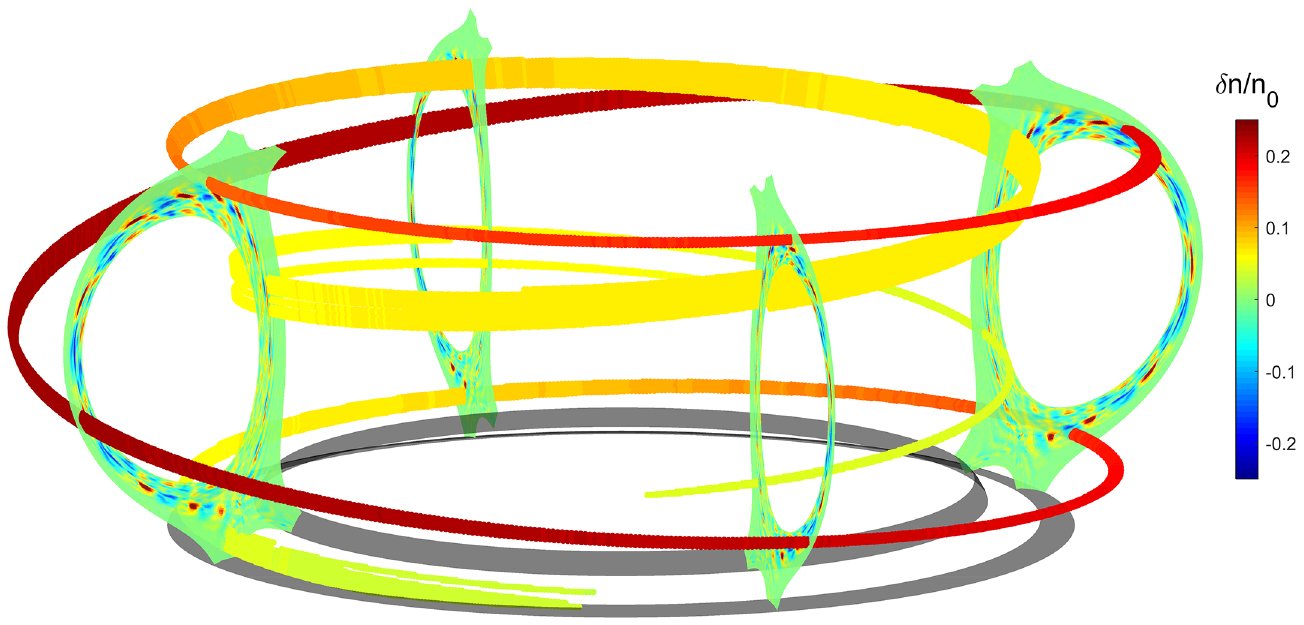
\includegraphics[width=0.9\linewidth]{Fig2_blob_movement.png}
        \normalsize{\caption{Density and movement of a blob with average density on the 4 poloidal planes \cite{nespoli_3d_2019}}}
        \label{fig:fig2}
    \end{subfigure}
    \normalsize{\caption{Simulations of a blob in tokamak plasmas}}
\end{figure}

\section*{Plan}
\subsection*{Plasma filament (blobs)}
\begin{itemize}
    \item What are plasma filaments
    \begin{itemize}
        \item Found in various magnetic fusion device, occurring in various regimes such as L and H mode \cite{boedo_transport_2003} and ELM mode \cite{ben_ayed_inter-elm_2009}
        \item Important as it affects particle transport and heat flux in SOL, and directly impacts durability and lifetime of plasma facing materials \cite{carralero_experimental_2015, krasheninnikov_recent_2008}
        \item Blob formation \cite{krasheninnikov_recent_2008}:
        \begin{enumerate}
            \item Turbulent processes (or MHD instabilities) causes plasma peel off at outmost layer (curvature and $\nabla$B induced F$\times$B drifts)
            \item Plasma polarization due to gravity drift
            \item Vertical charge separation induces E field ($\perp$ to toroidal B field)
            \item Plasma by E$\times$B force pushes blob towards chamber wall
        \end{enumerate}
        \item Large amount of 2D and 3D simulations \cite{omotani_effects_2015, easy_three_2014, nespoli_3d_2019, garcia_mechanism_2005, shanahan_fluid_2018} done to model blob structure and dynamic of blob to understand filament transport  
    \end{itemize}
    \item Blob equation
    \item Blob closures
\end{itemize}

\subsection*{Gaussian processes} 
\begin{itemize}
    \item What are Gaussian processes \cite{hornsby_gaussian_2024}
    \begin{itemize}    
        \item Machine learning method
        \item Reduced 'model' to predict results
    \end{itemize}
\end{itemize}

\nocite{*}
\printbibliography[title={References}]

\end{document}

